\chapter{Zásobníkové automaty}

Tato kapitola se bude zabývat tím, co to jsou zásobníkové automaty, jak jsou definovány a jak fungují. Zásobníkové automaty jsou jakýmsi rozšířením nedeterministických konečných automatů pro rozpoznávání bezkontextových gramatik. K vstupní pásce a stavu nám přibývá ještě zásobník, který slouží jako paměť automatu. % TODO: Popsat zásobník - LIFO

Příklad, kde bychom se bez zásobníku neobešli, je např.~automat kontrolující správné uzávorkování matematického výrazu. Při každém přečtení levé závorky si ji automat uloží na zásobník a při přečtení pravé závorky se zase podívá na zásobník, jestli tam má odpovídající levou závorku. V případě, že tam žádná závorka není nebo je tam závorka jiná, tak vstup není automatem přijat~---~není správně ozávorkován.

% TODO: Ukončit úvod

\section{Definice zásobníkových automatů}\label{sec:DefinitonOfPDA}

% BIB: https://fuuu.be/polytech/INFOF408/Introduction-To-The-Theory-Of-Computation-Michael-Sipser.pdf
Zásobníkový automat je formálně definován jako uspořádaná sedmice:\\
\indent\emph{$M = (Q, \Sigma, \Gamma, \delta, q_0, X_0, F)$}\\
kde $Q, \Sigma, \Gamma a F$ jsou neprázdné konečné množiny a 

\begin{itemize}
    \item $Q$ je množina stavů
    \item $\Sigma$ je vstupní abeceda
    \item $\Gamma$ je zásobníková abeceda
    \item $\delta \subseteq Q \times (\Sigma \cup \{\epsilon\}) \times \Gamma \rightarrow P(Q \times \Gamma^*)$ je přechodová funkce
    \item $q_0 \in Q$ je počáteční stav
    \item $X_0 \in \Gamma$ je počáteční zásobníkový symbol
    \item $F \subseteq Q$ je množina přijímacích/konečných stavů
\end{itemize}

% TODO: Popsat tři komponenty na obrázku a přepsat propojení s definicí výše
Graficky bychom mohli zásobníkový automat zobrazit jako na obrázku~\ref{fig:PDAComponents}. Množina stavů $Q$ obsahuje všechny stavy, ve kterých se může vyskytovat řídící jednotka při výpočtu. $\Sigma$ obsahuje všechny symboly, které se mohou vyskytnout na vstupní pásce a $\Gamma$ zase všechny symboly použitelné na zásobníku. $q_0$ je stav z množiny $Q$, ve kterém se nachází řídící jednotka na začátku výpočtu. $X_0$ je symbol z množiny $\Gamma$, který se nachází na zásobníku na začátku výpočtu. Množina $F$, která je podmnožinou $Q$, obsahuje všechny stavy, kterých je vstup přijat. $\delta$ obsahuje přechodové funkce, které mění stav automatu. Přechodová funkce $\delta : Q \times (\Sigma \cup \{\epsilon\}) \times \Gamma \rightarrow P(Q \times \Gamma^*)$ říká, jak se automat zachová při určitém stavu, když přečte vstupního symbolu a na vrcholu zásobníku je určitý symbol. Např.\ funkce $\delta(q_1,b,A) = \{(q_2,\{\epsilon\})\}$ říká, že pokud se ze vstupu přečte znak~$a$, na vrchu zásobníku je symbol~$A$ a řídící jednotka je ve stavu~$q_1$, tak se řídící jednotka přesune do stavu~$q_2$ a na zásobník se nic nepřidá.

\begin{figure}[h]
    \centering
    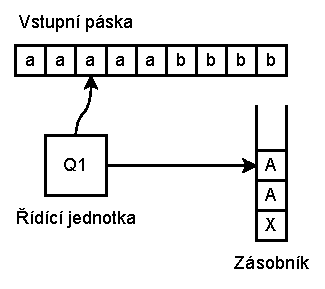
\includegraphics{Figures/PDAComponents.drawio.pdf}
    \caption{Grafické zobrazení zásobníkového automatu}\label{fig:PDAComponents}
\end{figure}

\section{Typu zásobníkových automatů}\label{sec:TypesOfPDA}

% BIB: https://www.geeksforgeeks.org/difference-between-npda-and-dpda/
Zásobníkové automaty stejně jako konečné automaty mohou být deterministické a nedeterministické. Pokud je automat deterministický, tak vždy musí existovat maximálně jedna funkce, která odpovídá aktuální konfiguraci automatu. Musí tedy splňovat tyto dvě podmínky:
\begin{enumerate}
    \item Pro kombinaci $(q,a,Z)$ může existovat maximálně jedna přechodová funkce
    \item Pokud existuje přechodová funkce $(q,\epsilon,Z)$, tak nesmí existovat žádná kombinace $(q,?,Z)$
\end{enumerate}
kde ($q \in Q$, $a \in \Sigma$ a $Z \in \Gamma$). Pokud pro kombinaci $(q,a,Z)$ existuje více než jedna přechodová funkce nebo navíc existuje ještě kombinace $(q,\epsilon,Z)$, jedná se o automat nedeterministický.

Definice použitá v kapitole~\ref{sec:DefinitonOfPDA} obsahuje podmnožinu stavů označovanou písmenem~F~---~množina přijímacích stavů. Pokud se po přečtení celého vstupu řídící jednotka nacházím v některém z přijímacích stavů, tak je vstup automatem přijat nezávisle na tom, jestli jsou nějaké symboly na zásobníku. V opačném případě tento automat vstup nepřijímá. Někdy ale můžeme chtít, aby bylo slovo přijato pouze, pokud je po přečtení celého slova zásobník prázdný. V tomto případě může být vhodnější zásobníkový automat (deterministický či nedeterministický) přijímající prázdným zásobníkem. Takový automat je definovaný jako šestice, neobsahuje množinu F, a po přečtení slova jej přijme, pokud na zásobníku není žádný symbol, nezávisle na stavu řídící jednotky.

Zásobníkové automaty se tedy dělí podle:
\begin{itemize}
    \item podmínek pro přechodové funkce na:
        \begin{itemize}
            \item deterministické
            \item nedeterministické
        \end{itemize}
    \item podle způsobu přijímání vstupu na:
        \begin{itemize}
            \item přijímající přijímacím stavem
            \item přijímající prázdným zásobníkem
        \end{itemize}
\end{itemize}

\section{Činnost zásobníkového automatu}

V kapitolách~\ref{sec:DefinitonOfPDA}~a~\ref{sec:TypesOfPDA} bylo popsáno, co to je zásobníkový automat, jak je definován a jaké jsou typy. Tato část se bude věnovat tomu, jak zásobníkový automat funguje a jak probíhá jeho činnost. Pro potřeby této kapitoly bude použit následný deterministický zásobníkový automat přijímající slovo prázdným zásobníkem rozpoznávající jazyk $a^{n}b^{n}, n \ge 1$:\\
$M = (Q, \Sigma, \Gamma, \delta, q, X)$, kde \\
\indent$Q = \{q\}$\\
\indent$\Sigma = \{a,b\}$\\
\indent$\Gamma = \{X,A\}$\\
\indent$\delta = \{$\\
\indent\indent$(q,a,X) \rightarrow (q,A)$,\\
\indent\indent$(q,a,A) \rightarrow (q,AA)$,\\
\indent\indent$(q,b,A) \rightarrow (q,\epsilon)$\\
\indent$\}$\\
Jako vstup bude použito slovo ``aaabbb''

% BIB: http://vishub.org/officedocs/13770.pdf strana 158 dole
V průběhu výpočtu se zásobníkový automat nachází vždy v nějaké konfiguraci, což je trojice $(Q \times \Sigma^{*} \times \Gamma^{*})$. $Q$ označuje aktuální stav, ve kterém se nachází řídící jednotka, $\Sigma^{*}$ nepřečtenou část vstupu a $\Gamma{*}$ aktuální stav zásobníku. 

Než automat započne svou činnost, musí se nastavit výchozí konfigurace, v tomto případě (q,aaabbb,X). 

Když automat začne výpočet, přečte první znak ze vstupu, tedy symbol a, ze zásobníku se odebere symbol X a řídící jednotka je ve stavu q. Automat tedy hledá přechodovou funkci pro trojici (q,a,X). Tomu odpovídá přechodová funkce (q,a,X), která se použije. Jelikož automat již je ve stavu q, stav zůstává stejný, čtecí hlava se na vstupu posune na další symbol a na zásobník se vloží znak A. Nově je automat v konfiguraci (q,aabbb,A). Tento postup se opakuje, dokud se nepřečte celý vstup, viz tabulka~\ref{tab:DemonstationOfPDA}. Po skončení výpočtu zůstal zásobník prázdný, je tedy slovo přijato. 

Pokud bychom měli vstup např.\ ``aaabb'', tak by výpočet vypadal obdobně, ale tabulka~\ref{tab:DemonstationOfPDA} byla končila řádkem s konfigurací (q,$\epsilon$,A) a žádnou přechodovou funkcí. Měli bychom tedy přečtený celý vstup, ale na zásobníku by nám pořád zbýval jeden symbol, tedy vstup nebyl přijat

% BIB: http://vishub.org/officedocs/13770.pdf strana 162
\begin{table}[h]
    \centering
    \begin{tabular}{c|c}
        Konfigurace zásobníkového automatu & Přechodová funkce \\
        \hline
        (q,aaabbb,X) & $(q,a,X) \rightarrow (q,A)$ \\
        (q,aabbb,A) & $(q,a,A) \rightarrow (q,AA)$ \\
        (q,abbb,AA) & $(q,a,A) \rightarrow (q,AA)$ \\
        (q,bbb,AAA) & $(q,b,A) \rightarrow (q,\epsilon)$ \\
        (q,bb,AA) & $(q,b,A) \rightarrow (q,\epsilon)$ \\
        (q,b,A) & $(q,b,A) \rightarrow (q,\epsilon)$ \\
        (q,$\epsilon$,$\epsilon$) &  \\
    \end{tabular}
    \caption{Ukázka činnosti zásobníkového automatu }\label{tab:DemonstationOfPDA}
\end{table}

\endinput